\documentclass{article}
\usepackage{graphicx}
\usepackage{subcaption}
\usepackage{booktabs}
\usepackage{array}
\usepackage{geometry}
\geometry{margin=1in}
\usepackage{amsmath}
\usepackage{booktabs}

\begin{document}

\begin{figure}[ht]
  \centering
  \begin{subfigure}{0.3\textwidth}
    \centering
    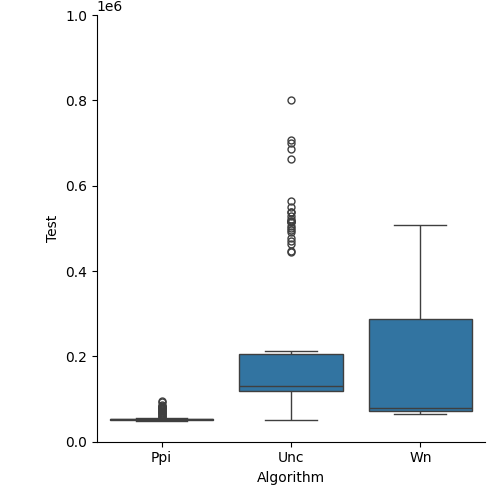
\includegraphics[width=\linewidth]{../figureIntRandom100.png}
    \caption{Size: 100}
    \label{fig:img1}
  \end{subfigure}
  \begin{subfigure}{0.3\textwidth}
    \centering
    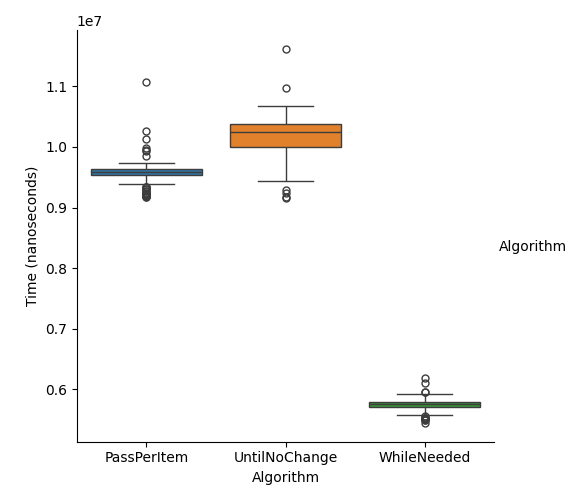
\includegraphics[width=\linewidth]{../figureIntRandom1000.png}
    \caption{Size 1000}
    \label{fig:img2}
  \end{subfigure}
  \begin{subfigure}{0.3\textwidth}
    \centering
    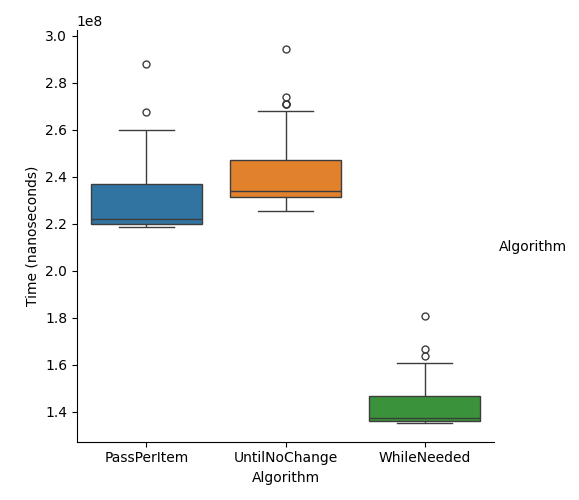
\includegraphics[width=\linewidth]{../figureIntRandom5000.png}
    \caption{Size 5000}
    \label{fig:img3}
  \end{subfigure}
  \caption{Time to sort array of random Integers}
  \label{fig:three_images}
\end{figure}

\begin{figure}[ht]
  \centering
  \begin{subfigure}{0.3\textwidth}
    \centering
    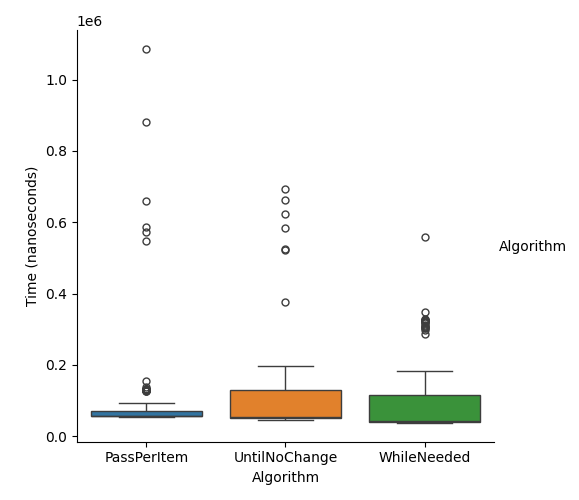
\includegraphics[width=\linewidth]{../figureByteRandom100.png}
    \caption{Size: 100}
    \label{fig:img1}
  \end{subfigure}
  \begin{subfigure}{0.3\textwidth}
    \centering
    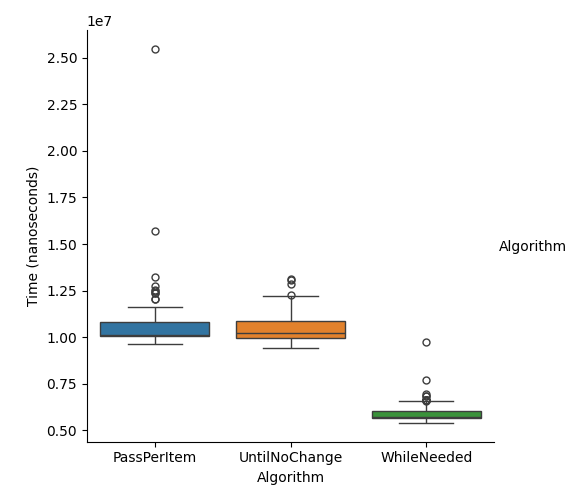
\includegraphics[width=\linewidth]{../figureByteRandom1000.png}
    \caption{Size 1000}
    \label{fig:img2}
  \end{subfigure}
  \begin{subfigure}{0.3\textwidth}
    \centering
    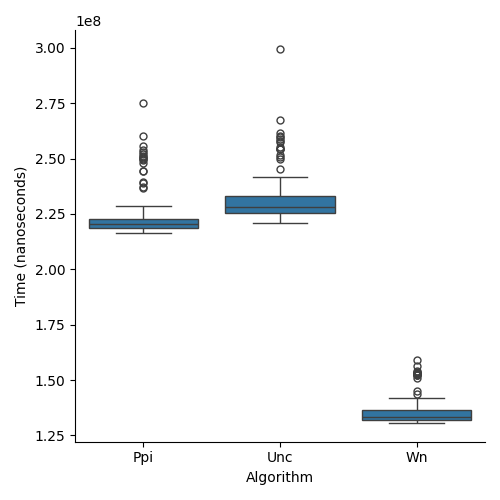
\includegraphics[width=\linewidth]{../figureByteRandom5000.png}
    \caption{Size 5000}
    \label{fig:img3}
  \end{subfigure}
  \caption{Time to sort random array of Bytes}
  \label{fig:three_images}
\end{figure}

\begin{figure}[ht]
  \centering
  \begin{subfigure}{0.3\textwidth}
    \centering
    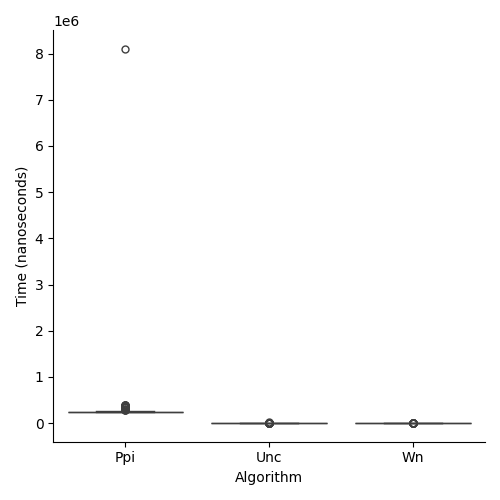
\includegraphics[width=\linewidth]{../figureStringRandom100.png}
    \caption{Size: 100}
    \label{fig:img1}
  \end{subfigure}
  \begin{subfigure}{0.3\textwidth}
    \centering
    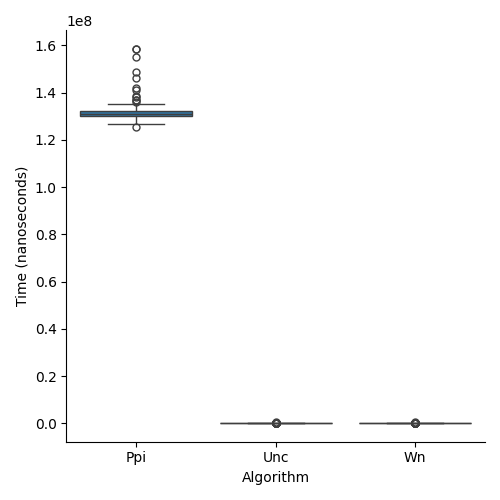
\includegraphics[width=\linewidth]{../figureStringRandom1000.png}
    \caption{Size 1000}
    \label{fig:img2}
  \end{subfigure}
  \begin{subfigure}{0.3\textwidth}
    \centering
    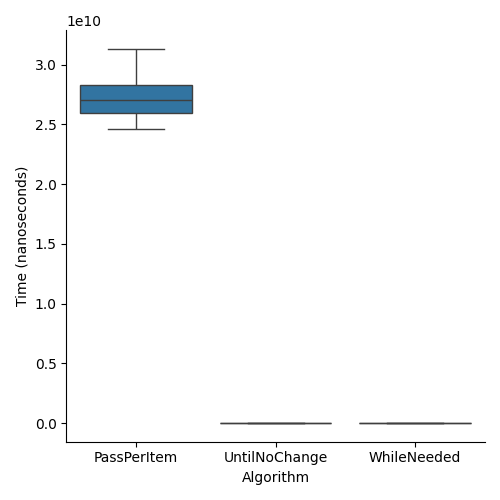
\includegraphics[width=\linewidth]{../figureStringRandom5000.png}
    \caption{Size 5000}
    \label{fig:img3}
  \end{subfigure}
  \caption{Time to sort random array of String}
  \label{fig:three_images}
\end{figure}

\begin{table}[htbp]
    \centering
    \begin{tabular}{ccccccc}
        \toprule
        \textbf{Size} & \textbf{Algorithm} & \textbf{Minimum} & \textbf{First Quartile} & \textbf{Median} & \textbf{Third Quartile} & \textbf{Maximum} \\
        \midrule
        100 & PassPerItem & 49.85 & 50.07 & 50.31 & 50.82 & 87.38 \\
        100 & UntilNoChange & 56.74 & 56.92 & 57.06 & 57.45 & 103.16 \\
        100 & WhileNeeded & 33.44 & 33.50 & 33.59 & 33.78 & 69.36 \\
        1000 & PassPerItem & 9606.17 & 9640.39 & 9665.68 & 9751.96 & 31493.50 \\
        1000 & UntilNoChange & 9548.54 & 9562.60 & 9575.98 & 9774.66 & 31540.57 \\
        1000 & WhileNeeded & 5481.91 & 5497.36 & 5507.04 & 5569.73 & 17908.92 \\
        5000 & PassPerItem & 208339.31 & 210349.57 & 212377.40 & 219466.91 & 263363.72 \\
        5000 & UntilNoChange & 210984.56 & 211619.51 & 214544.31 & 227371.03 & 298996.13 \\
        5000 & WhileNeeded & 122377.71 & 122787.50 & 124621.14 & 132163.16 & 173597.92 \\
        \bottomrule
    \end{tabular}
    \caption{Performance Metrics for arrays of Descending Integers (in microseconds)}
    \label{tab:performance}
\end{table}

\begin{table}[htbp]
    \centering
    \begin{tabular}{ccccccc}
        \toprule
        \textbf{Size} & \textbf{Algorithm} & \textbf{Minimum} & \textbf{First Quartile} & \textbf{Median} & \textbf{Third Quartile} & \textbf{Maximum} \\
        \midrule
        100 & PassPerItem & 58.54 & 58.77 & 58.96 & 59.42 & 99.76 \\
        100 & UntilNoChange & 57.71 & 58.16 & 58.32 & 58.76 & 104.34 \\
        100 & WhileNeeded & 42.91 & 43.02 & 43.13 & 43.43 & 75.81 \\
        1000 & PassPerItem & 9548.90 & 9708.79 & 9747.38 & 9877.97 & 17988.70 \\
        1000 & UntilNoChange & 9859.16 & 10082.39 & 10124.00 & 10387.20 & 17207.29 \\
        1000 & WhileNeeded & 5687.05 & 5857.50 & 5881.01 & 5975.96 & 14572.42 \\
        5000 & PassPerItem & 205850.43 & 209231.70 & 211795.54 & 214074.12 & 241904.37 \\
        5000 & UntilNoChange & 215364.05 & 216803.60 & 219137.71 & 222237.53 & 249848.90 \\
        5000 & WhileNeeded & 123721.80 & 125714.37 & 126542.95 & 129139.10 & 151971.81 \\
        \bottomrule
    \end{tabular}
    \caption{Performance Metrics for arrays of Descending Bytes(in microseconds)}
    \label{tab:performance_2}
\end{table}

\begin{table}[htbp]
    \centering
    \begin{tabular}{ccccccc}
        \toprule
        \textbf{Size} & \textbf{Algorithm} & \textbf{Minimum} & \textbf{First Quartile} & \textbf{Median} & \textbf{Third Quartile} & \textbf{Maximum} \\
        \midrule
        100 & PassPerItem & 250.51 & 260.69 & 262.30 & 264.39 & 361.71 \\
        100 & UntilNoChange & 252.84 & 264.19 & 265.84 & 268.57 & 300.53 \\
        100 & WhileNeeded & 121.71 & 126.99 & 127.92 & 129.11 & 158.24 \\
        1000 & PassPerItem & 117837.06 & 119357.54 & 121274.97 & 123099.46 & 143828.36 \\
        1000 & UntilNoChange & 117809.62 & 119980.49 & 121655.67 & 123569.40 & 140236.91 \\
        1000 & WhileNeeded & 45292.69 & 45868.37 & 46430.09 & 47424.17 & 57093.29 \\
        5000 & PassPerItem & 25781857.71 & 26383544.20 & 26828103.50 & 27380123.07 & 29426932.85 \\
        5000 & UntilNoChange & 25842208.87 & 26413720.27 & 26818579.97 & 27416407.67 & 29207443.63 \\
        5000 & WhileNeeded & 8228578.19 & 8406592.12 & 8543826.54 & 8635735.72 & 9775953.45 \\
        \bottomrule
    \end{tabular}
    \caption{Performance Metrics for arrays of Descending Strings(in microseconds)}
    \label{tab:performance_4}
\end{table}

\begin{table}[htbp]
    \centering
    \begin{tabular}{ccccccc}
        \toprule
        \textbf{Size} & \textbf{Algorithm} & \textbf{Minimum} & \textbf{First Quartile} & \textbf{Median} & \textbf{Third Quartile} & \textbf{Maximum} \\
        \midrule
        100 & PassPerItem & 31.47 & 31.64 & 31.71 & 31.84 & 47.30 \\
        100 & UntilNoChange & 0.46 & 0.51 & 0.53 & 0.55 & 1.28 \\
        100 & WhileNeeded & 0.42 & 0.47 & 0.49 & 0.50 & 1.05 \\
        1000 & PassPerItem & 7913.74 & 7981.70 & 8007.96 & 8041.87 & 8261.34 \\
        1000 & UntilNoChange & 8.72 & 8.83 & 8.95 & 9.11 & 13.34 \\
        1000 & WhileNeeded & 8.60 & 8.72 & 8.78 & 8.97 & 10.79 \\
        5000 & PassPerItem & 172160.11 & 172462.95 & 175633.39 & 179902.05 & 223133.42 \\
        5000 & UntilNoChange & 37.61 & 37.76 & 37.99 & 39.33 & 46.91 \\
        5000 & WhileNeeded & 37.06 & 37.18 & 37.39 & 38.58 & 69.91 \\
        \bottomrule
    \end{tabular}
    \caption{Performance Metrics for array of Ascending Integers (in microseconds)}
    \label{tab:performance_5}
\end{table}

\begin{table}[htbp]
    \centering
    \begin{tabular}{ccccccc}
        \toprule
        \textbf{Size} & \textbf{Algorithm} & \textbf{Minimum} & \textbf{First Quartile} & \textbf{Median} & \textbf{Third Quartile} & \textbf{Maximum} \\
        \midrule
        100 & PassPerItem & 33.12 & 33.17 & 33.22 & 39.41 & 61.92 \\
        100 & UntilNoChange & 0.39 & 0.41 & 0.44 & 0.65 & 1.10 \\
        100 & WhileNeeded & 0.42 & 0.46 & 0.50 & 0.65 & 1.09 \\
        1000 & PassPerItem & 7829.75 & 7881.66 & 7900.80 & 8243.30 & 14010.38 \\
        1000 & UntilNoChange & 8.63 & 8.81 & 8.91 & 9.25 & 16.23 \\
        1000 & WhileNeeded & 8.51 & 8.67 & 8.79 & 9.12 & 16.05 \\
        5000 & PassPerItem & 170007.62 & 171708.70 & 173837.23 & 179121.64 & 200752.12 \\
        5000 & UntilNoChange & 36.90 & 37.19 & 38.38 & 39.96 & 43.44 \\
        5000 & WhileNeeded & 36.48 & 36.74 & 37.92 & 39.49 & 44.25 \\
        \bottomrule
    \end{tabular}
    \caption{Performance Metrics for array of Ascending Bytes (in microseconds)}
    \label{tab:performance_6}
\end{table}

\begin{table}[htbp]
    \centering
    \begin{tabular}{ccccccc}
        \toprule
        \textbf{Size} & \textbf{Algorithm} & \textbf{Minimum} & \textbf{First Quartile} & \textbf{Median} & \textbf{Third Quartile} & \textbf{Maximum} \\
        \midrule
        100 & PassPerItem & 2344.88 & 2370.67 & 2390.62 & 2451.50 & 3925.87 \\
        100 & UntilNoChange & 2.70 & 2.78 & 2.84 & 3.01 & 5.40 \\
        100 & WhileNeeded & 2.66 & 2.73 & 2.78 & 2.89 & 5.44 \\
        1000 & PassPerItem & 110443.20 & 113969.67 & 116479.11 & 126305.95 & 150915.52 \\
        1000 & UntilNoChange & 1115.18 & 1148.30 & 1188.21 & 1301.90 & 1387.19 \\
        1000 & WhileNeeded & 1116.18 & 1148.61 & 1179.82 & 1278.60 & 1837.99 \\
        5000 & PassPerItem & 24684319.39 & 25299065.33 & 25882470.86 & 26998749.87 & 30100566.89 \\
        5000 & UntilNoChange & 4821.40 & 5035.65 & 5165.47 & 5373.65 & 6121.47 \\
        5000 & WhileNeeded & 4843.33 & 5020.98 & 5167.28 & 5404.01 & 5865.17 \\
        \bottomrule
    \end{tabular}
    \caption{Performance Metrics for arrays of Ascending Strings (in microseconds)}
    \label{tab:performance_7}
\end{table}

\begin{figure}[ht]
  \centering
  \begin{subfigure}{0.3\textwidth}
    \centering
    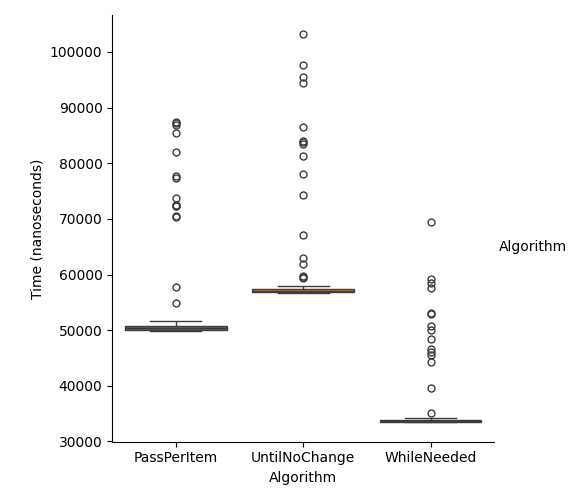
\includegraphics[width=\linewidth]{../figureIntDesc100.png}
    \caption{Size: 100}
    \label{fig:img1}
  \end{subfigure}
  \begin{subfigure}{0.3\textwidth}
    \centering
    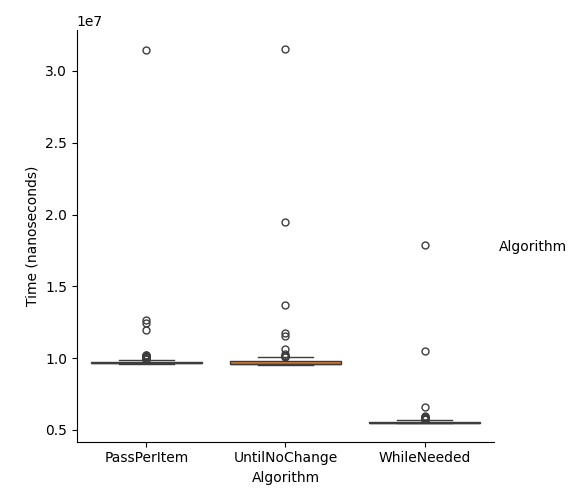
\includegraphics[width=\linewidth]{../figureIntDesc1000.png}
    \caption{Size 1000}
    \label{fig:img2}
  \end{subfigure}
  \begin{subfigure}{0.3\textwidth}
    \centering
    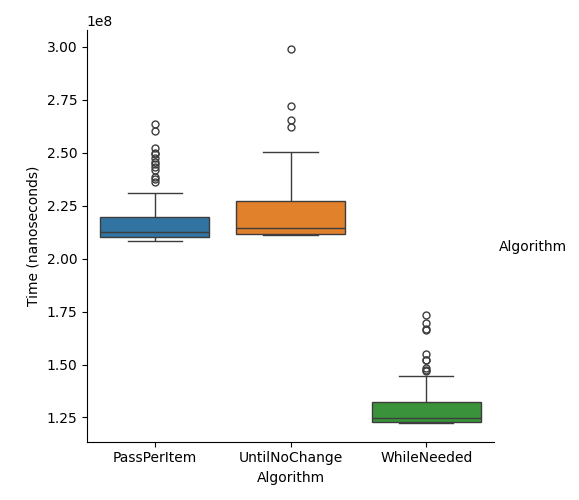
\includegraphics[width=\linewidth]{../figureIntDesc5000.png}
    \caption{Size 5000}
    \label{fig:img3}
  \end{subfigure}
  \caption{Time to sort descending of random Integers}
  \label{fig:three_images}
\end{figure}

\begin{figure}[ht]
  \centering
  \begin{subfigure}{0.3\textwidth}
    \centering
    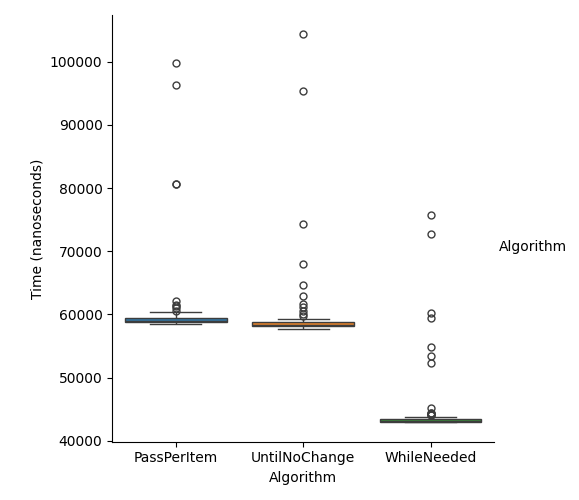
\includegraphics[width=\linewidth]{../figureByteDesc100.png}
    \caption{Size: 100}
    \label{fig:img1}
  \end{subfigure}
  \begin{subfigure}{0.3\textwidth}
    \centering
    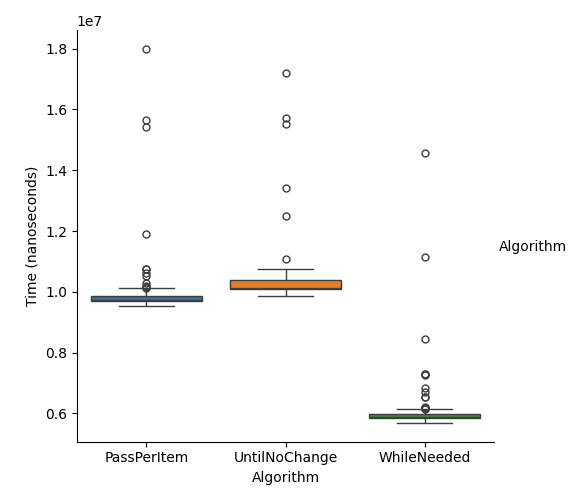
\includegraphics[width=\linewidth]{../figureByteDesc1000.png}
    \caption{Size 1000}
    \label{fig:img2}
  \end{subfigure}
  \begin{subfigure}{0.3\textwidth}
    \centering
    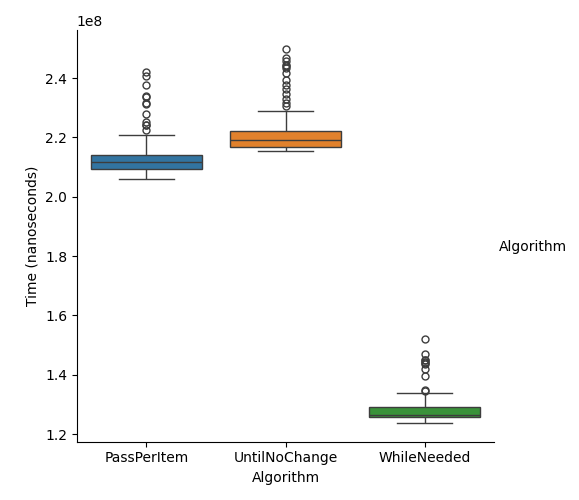
\includegraphics[width=\linewidth]{../figureByteDesc5000.png}
    \caption{Size 5000}
    \label{fig:img3}
  \end{subfigure}
  \caption{Time to sort descending array of Bytes}
  \label{fig:three_images}
\end{figure}

\begin{figure}[ht]
  \centering
  \begin{subfigure}{0.3\textwidth}
    \centering
    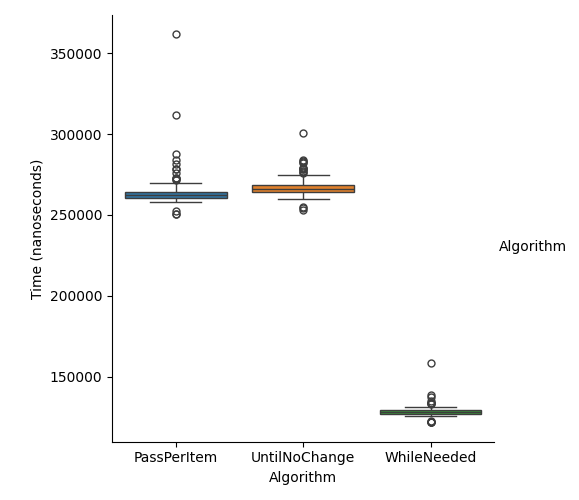
\includegraphics[width=\linewidth]{../figureStringDesc100.png}
    \caption{Size: 100}
    \label{fig:img1}
  \end{subfigure}
  \begin{subfigure}{0.3\textwidth}
    \centering
    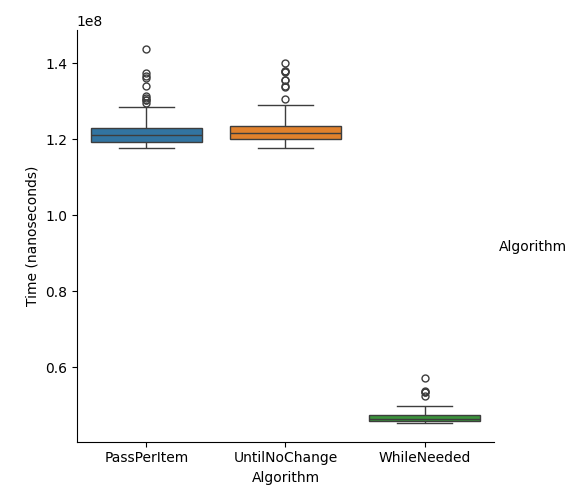
\includegraphics[width=\linewidth]{../figureStringDesc1000.png}
    \caption{Size 1000}
    \label{fig:img2}
  \end{subfigure}
  \begin{subfigure}{0.3\textwidth}
    \centering
    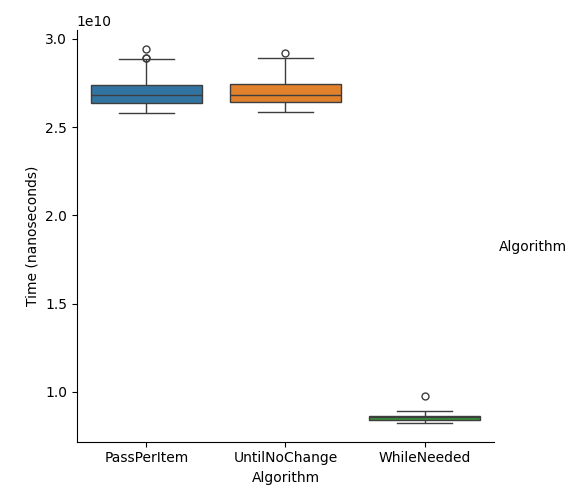
\includegraphics[width=\linewidth]{../figureStringDesc5000.png}
    \caption{Size 5000}
    \label{fig:img3}
  \end{subfigure}
  \caption{Time to sort descending array of String}
  \label{fig:three_images}
\end{figure}

\begin{figure}[ht]
  \centering
  \begin{subfigure}{0.3\textwidth}
    \centering
    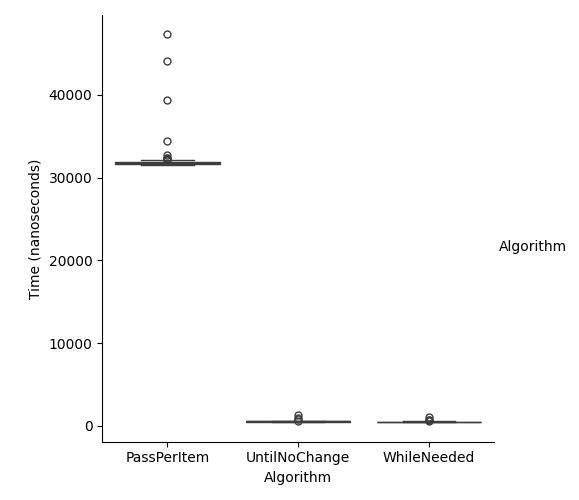
\includegraphics[width=\linewidth]{../figureIntAsc100.png}
    \caption{Size: 100}
    \label{fig:img1}
  \end{subfigure}
  \begin{subfigure}{0.3\textwidth}
    \centering
    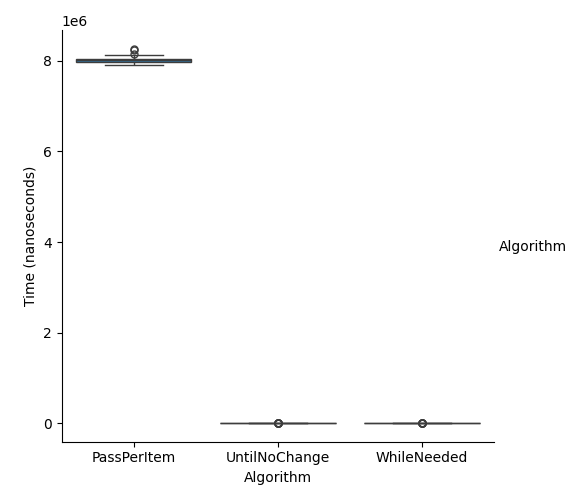
\includegraphics[width=\linewidth]{../figureIntAsc1000.png}
    \caption{Size 1000}
    \label{fig:img2}
  \end{subfigure}
  \begin{subfigure}{0.3\textwidth}
    \centering
    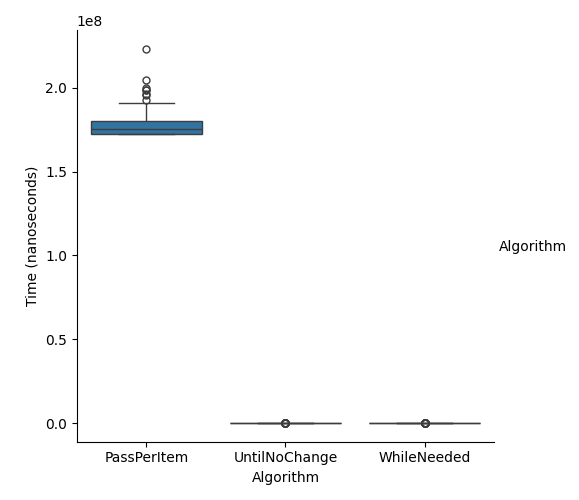
\includegraphics[width=\linewidth]{../figureIntAsc5000.png}
    \caption{Size 5000}
    \label{fig:img3}
  \end{subfigure}
  \caption{Time to sort ascending of random Integers}
  \label{fig:three_images}
\end{figure}

\begin{figure}[ht]
  \centering
  \begin{subfigure}{0.3\textwidth}
    \centering
    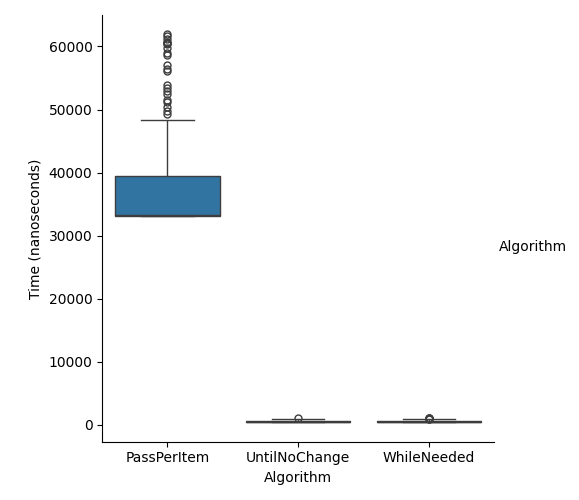
\includegraphics[width=\linewidth]{../figureByteAsc100.png}
    \caption{Size: 100}
    \label{fig:img1}
  \end{subfigure}
  \begin{subfigure}{0.3\textwidth}
    \centering
    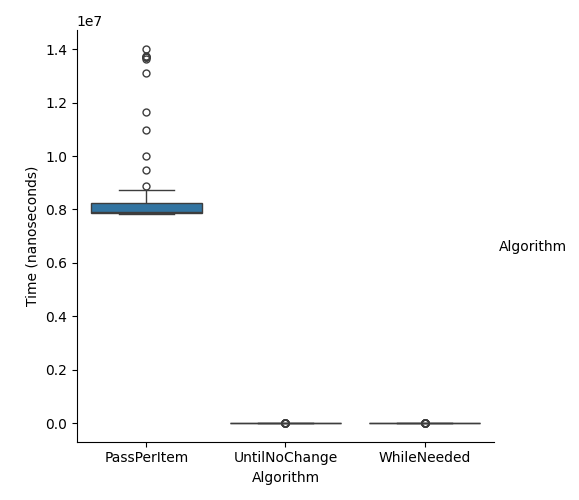
\includegraphics[width=\linewidth]{../figureByteAsc1000.png}
    \caption{Size 1000}
    \label{fig:img2}
  \end{subfigure}
  \begin{subfigure}{0.3\textwidth}
    \centering
    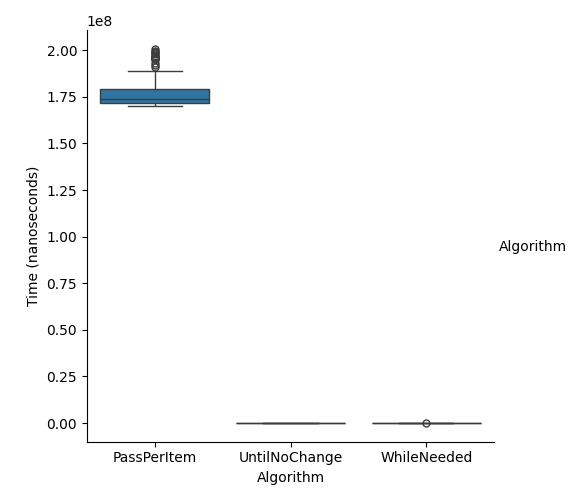
\includegraphics[width=\linewidth]{../figureByteAsc5000.png}
    \caption{Size 5000}
    \label{fig:img3}
  \end{subfigure}
  \caption{Time to sort ascending array of Bytes}
  \label{fig:three_images}
\end{figure}

\begin{figure}[ht]
  \centering
  \begin{subfigure}{0.3\textwidth}
    \centering
    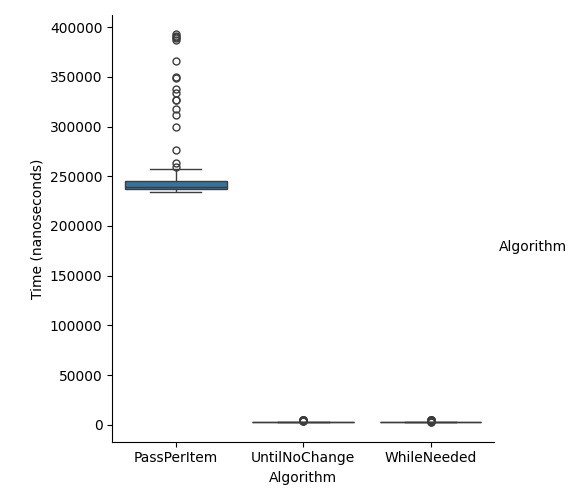
\includegraphics[width=\linewidth]{../figureStringAsc100.png}
    \caption{Size: 100}
    \label{fig:img1}
  \end{subfigure}
  \begin{subfigure}{0.3\textwidth}
    \centering
    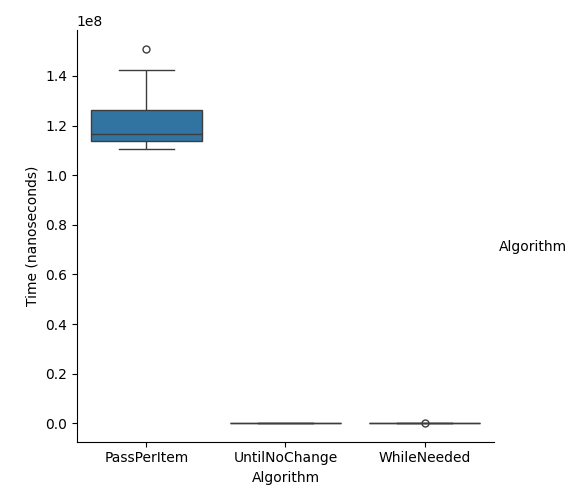
\includegraphics[width=\linewidth]{../figureStringAsc1000.png}
    \caption{Size 1000}
    \label{fig:img2}
  \end{subfigure}
  \begin{subfigure}{0.3\textwidth}
    \centering
    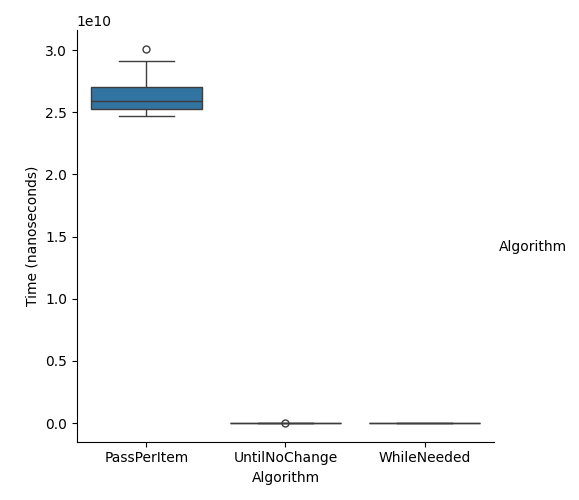
\includegraphics[width=\linewidth]{../figureStringAsc5000.png}
    \caption{Size 5000}
    \label{fig:img3}
  \end{subfigure}
  \caption{Time to sort ascending array of String}
  \label{fig:three_images}
\end{figure}

\end{document}
